\documentclass{article}
\usepackage{latexsym}
\usepackage{amssymb,amsmath}
\usepackage{custom2}
\usepackage{graphicx} % for figures
\usepackage{epstopdf} % so can use EPS or PDF figures
\usepackage{caption}
\usepackage{subcaption}
\usepackage{url}
\usepackage{amssymb,amsfonts}
\usepackage[all,arc]{xy}
\usepackage{enumerate}
\usepackage{mathrsfs}
\usepackage{booktabs}
\usepackage[pdftex]{hyperref}
\usepackage{lscape}
\captionsetup{justification=RaggedRight, singlelinecheck=false}
\newcommand{\ra}[1]{\renewcommand{\arraystretch}{#1}}
\newcommand{\argmax}{\text{argmax}}
\newcommand{\Tr}{\text{Tr}}
%\newtheorem{claim}{Claim}
\newtheorem{ass}{Assumption}

\addtolength{\evensidemargin}{-.5in}
\addtolength{\oddsidemargin}{-.5in}
\addtolength{\textwidth}{1.4in}
\addtolength{\textheight}{1.4in}
\addtolength{\topmargin}{-.5in}


\pagestyle{empty}

\begin{document}
\begin{center}
\Large

\end{center}


\vspace{0pt}

\begin{center}
{\bf \LARGE{Development of a Signaling Network}}
\vspace{10pt}
\\ Eleanor Brush 
\\ updated December 12, 2012
\end{center}

\tableofcontents

\vspace{0pt}
\normalsize

\section{Introduction}
In some species of macaques, there is a stereotyped signal that one animal emits to another once it has learned, through a series of fights, that it is likely to lose subsequent fights.  The signal communicates the signaler's agreement to the subordinate role in the relationship.  The animals then use the signals they observe being transmitted between other pairs of animals in the group to estimate the relative power of the other group members.  In different species of macaque, the network of signals transmitted between every pair and power distribution are more or less skewed.  I have previously worked on ways to measure the amount of consensus present in an observed signaling network.  I am now studying the development of the signaling network.  I am developing and starting to analyze a model of stochastic fighting and signaling dynamics.  Using this model, I hope to be able to understand under what circumstances the animals should or should not signal and to explain how the traits of the individuals and the distribution of these traits in the group affect the resulting signaling network.  From encounters, fights, and signals that occur probabilistically, I can simulate and derive stochastic differential equations describing how each animal's estimate of its relative ability changes over time (Equation \ref{sdes}).   From these equations I can find the expected time until one animal signals and the probability that one or the other animal will be the first to signal.  I can then find the thresholds that optimize these pairwise dynamics and how that optimization affects the resulting network of signals among the whole population.  Many scientists have used this kind of drift-diffusion model to describe learning dynamics in neurons.  People have made analogies between social systems and networks of neurons and I would like to use this model to explore the analogy, identifying similarities, studying the consequences of differences in the dynamics, and hopefully probing the limits to which the analogy can be pushed.  The possibility of the animals or neurons communicating with each other represents a feedback between the variables not present in most models of neuronal learning and I am interested in understanding, generally, what the effect of this feedback is on the ability of individuals and groups of individuals to learn about each other and their environment.

This model is interesting for (at least) two reasons.  First, we hope to be able to explain variation we see at the group or species level in primates, namely characteristic signaling behavior and signaling networks, with differences in individual level properties, distributions of those properties, and the varying benefits or costs of fighting and storing information, i.e. to use individual level variation to explain emergent properties of species.  Second, we hope to use this model as a tool to explore the analogy between neural and social systems.

\section{Stochastic Model}
\subsection{Derivation of Stochastic Differential Equations}
We want to write down equations for how the two animal's estimates of their dominance change over time.  We assume that in the absence of any information, an animal's belief about its own dominance leaks back towards $0$ with rate $\ell$.  (A table of all variables used in the text is given in Table \ref{variables}.) If nothing else happened, then over a period of time of length $\tau$ an estimate would decrease as $X(t+\tau)=(1-\ell\tau)X(t)$; consequently $X(t)=\exp(-\ell t)$. Two things can happen to change an animal's estimate: it can receive a signal, boosting its estimate, or it can engage in a fight and learn about its relative dominance from the outcome of the fight.  To determine the estimate at time $t+\tau$, we can count how many times each of these events occurred in the time since $t$ and add the changes resulting from these events to the background leaky estimate (as in \cite{Gillespie:2000fk}):
\begin{align*}
X(t+\tau)&=(1-\ell\tau)X(t)+b_{\text{s}}\times\# \text{ of signals received in }[t,t+\tau)
\\&+b_{\text{f}}\times\#\text{ of fights won in }[t,t+\tau)-b_{\text{f}}\times\#\text{ of fights lost in }[t,t+\tau)
\end{align*}


The animals encounter each other at a constant rate over time.  When the animals encounter each other, each animal has a probability of transmitting a signal.  (We do not preclude the possibility of both animals signaling.)  If no signals are transmitted, then the encounter will escalate to a fight with some probability.  If the animals fight, the probability that the ``stronger" animal will win is determined by how much stronger or more ``dominant" he is.  We write $N_{\text{s},i}$ for the random variable giving the number of signals transmitted by animal $i$ and $N_{\text{f},i}$ for the random variable giving the number of fights won by animal $i$.  This very general description of our model is sufficient to perform simulations of these stochastic processes.  To write down equations for the probability densities of the estimates, however, we make a few assumptions.

If the rates at which the pair of animals encounters each other, fight with each other, and signal to each other do not change from $t$ to $t+\tau$ then the numbers of these events follow Poisson distributions, as shown in the Appendix.  
\begin{ass}
There is a timescale $\tau$ over which the probabilities of the animals encountering each other, engaging in fights with each other, and transmitting signals do not change.
\end{ass}

Putting this all together gives that 
\begin{align*}
X_1(t+\tau)&=(1-\ell\tau)X_1(t)+b_{\text{s}}N_{\text{s},2}+b_{\text{f}}N_{\text{f},1}-b_{\text{f}}N_{\text{f},2}
\\ \text{ and } X_2(t+\tau)&=(1-\ell\tau)X_2(t)+b_{\text{s}}N_{\text{s},1}-b_{\text{f}}N_{\text{f},1}+b_{\text{f}}N_{\text{f},2}.
\end{align*}
Somewhat counterintuitively, even though the transmission of a signal and a fight are mutually exclusive types of encounters, the numbers of these events are independent random variables, each following a Poisson distribution, as shown in the Appendix.  $N_{\text{s},1}$, $N_{\text{s},2}$, $N_{\text{f},1}$ and $N_{\text{f},1}$ are therefore independent Poisson random variables with respective means $\tau ep_{\text{s},1}(t)$, $\tau ep_{\text{s},2}(t)$, $\tau e(1-p_{\text{s},1}(t))(1-p_{\text{s},2}(t))p_{\text{f}}d$, and $\tau e(1-p_{\text{s},1}(t))(1-p_{\text{s},2}(t))p_{\text{f}}(1-d)$.  If enough events happen in the period of time from $t$ to $t+\tau$ then we can approximate the Poisson random variables with Normal random variables with mean and variance equal to the mean of the Poisson random variables.

\begin{ass}
In the period of time of length $\tau$ enough events happen that we can approximate the Poisson random variables with normally distributed random variables.
\end{ass}
Let $Z_{\text{s},1}$, $Z_{\text{s},2}$, $Z_{\text{f},1}$, and $Z_{\text{f},2}$ be independent standard Normal random variables, i.e. with mean $0$ and standard deviation $1$.  Then our equations for $X_i(t+\tau)$ become
\begin{align*}
X_1(t+\tau)&=(1-\ell\tau)X_1(t)+b_{\text{s}}\bigg(\tau ep_{\text{s},2}(t)+\sqrt{\tau ep_{\text{s},2}(t)}Z_{\text{s},2}\bigg)
\\&+b_{\text{f}}\bigg(\tau e(1-p_{\text{s},1}(t))(1-p_{\text{s},2}(t))p_{\text{f}}d+\sqrt{\tau e(1-p_{\text{s},1}(t))(1-p_{\text{s},2}(t))p_{\text{f}}d}Z_{\text{f},1}\bigg)
\\&-b_{\text{f}}\bigg(\tau e(1-p_{\text{s},1}(t))(1-p_{\text{s},2}(t))p_{\text{f}}(1-d)+\sqrt{\tau e(1-p_{\text{s},1}(t))(1-p_{\text{s},2}(t))p_{\text{f}}(1-d)}Z_{\text{f},2}\bigg),
\\ \text{ and } X_2(t+\tau)&=(1-\ell\tau)X_2(t)+b_{\text{s}}\bigg(\tau ep_{\text{s},1}(t)+\sqrt{\tau ep_{\text{s},1}(t)}Z_{\text{s},2}\bigg)
\\&-b_{\text{f}}\bigg(\tau e(1-p_{\text{s},1}(t))(1-p_{\text{s},2}(t))p_{\text{f}}d+\sqrt{\tau e(1-p_{\text{s},1}(t))(1-p_{\text{s},2}(t))p_{\text{f}}d}Z_{\text{f},1}\bigg)
\\&+b_{\text{f}}\bigg(\tau e(1-p_{\text{s},1}(t))(1-p_{\text{s},2}(t))p_{\text{f}}(1-d)+\sqrt{\tau e(1-p_{\text{s},1}(t))(1-p_{\text{s},2}(t))p_{\text{f}}(1-d)}Z_{\text{f},2}\bigg).
\end{align*}
Finally, as we make the period of time shorter and shorter, making $\tau$ infinitesimally small, these equations become stochastic differential equations,
\begin{equation}
\begin{array}{ll}
dX_1&=\bigg(-\ell X_1(t)+b_{\text{s}}ep_{\text{s},2}(t)+b_{\text{f}}(2d-1)e(1-p_{\text{s},1}(t))(1-p_{\text{s},2}(t))p_\text{f}\bigg)dt+b_{\text{s}}\sqrt{ep_{\text{s},2}(t)}dW_{\text{s},2}t
\\&+b_f\sqrt{e(1-p_{\text{s},1}(t))(1-p_{\text{s},2}(t))p_{\text{f}}d}dW_{\text{f},1}t-b_{\text{f}}\sqrt{e(1-p_{\text{s},1}(t))(1-p_{\text{s},2}(t))p_{\text{f}}(1-d)}dW_{\text{f},2}t
\\dX_2&=\bigg(-\ell X_2(t)+b_{\text{s}}ep_{\text{s},1}(t)+b_{\text{f}}(1-2d)e(1-p_{\text{s},1}(t))(1-p_{\text{s},2}(t))p_\text{f}\bigg)dt+b_{\text{s}}\sqrt{ep_{\text{s},1}(t)}dW_{\text{s},1}t
\\&-b_f\sqrt{e(1-p_{\text{s},1}(t))(1-p_{\text{s},2}(t))p_{\text{f}}d}dW_{\text{f},1}t+b_{\text{f}}\sqrt{e(1-p_{\text{s},1}(t))(1-p_{\text{s},2}(t))p_{\text{f}}(1-d)}dW_{\text{f},2}t,
\end{array}
\end{equation}
where $dW_{\text{s},i}$ and $dW_{\text{f},i}$ and independent Brownian motions representing, respectively, the signaling of animal $i$ and animal $i$ winning fights.

\begin{table}
\caption{\label{variables}}
\begin{tabular}{llll}
Variable & Meaning  \\
\hline $e$ & encounter rate
\\ $p_{\text{s},i}(t)$ & probability of animal $i$ transmitting a signal as a function of the animal's estimate at $t$
\\ $p_{\text{f}}$ & probability of fighting
\\ $d$ & probability of stronger animal winning (``dominance'')
\\ $b_{\text{s}}$ & boost to one's estimate from receiving a signal
\\ $b_{\text{f}}$ & boost to one's estimate from winning a fight
\\ $\ell$ & leak or loss rate
\end{tabular}
\end{table}

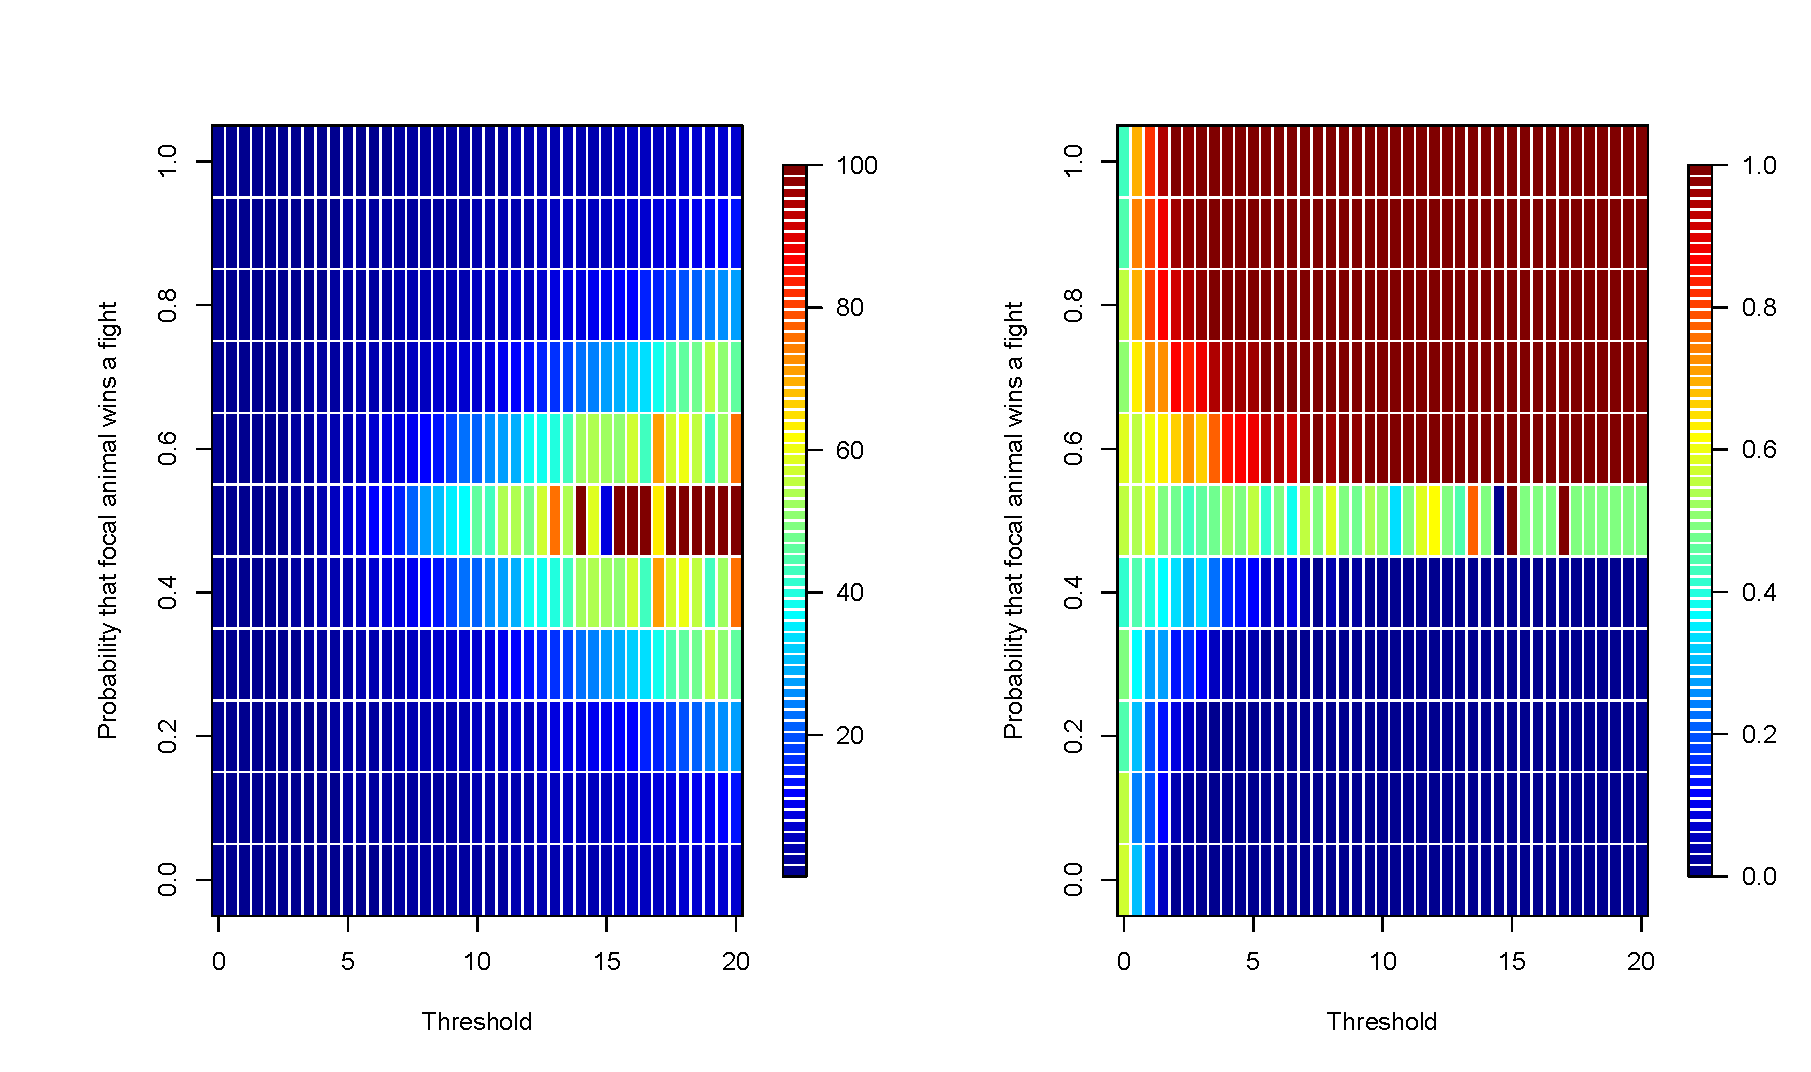
\includegraphics[width=\linewidth]{figures/prelim_stats.pdf}
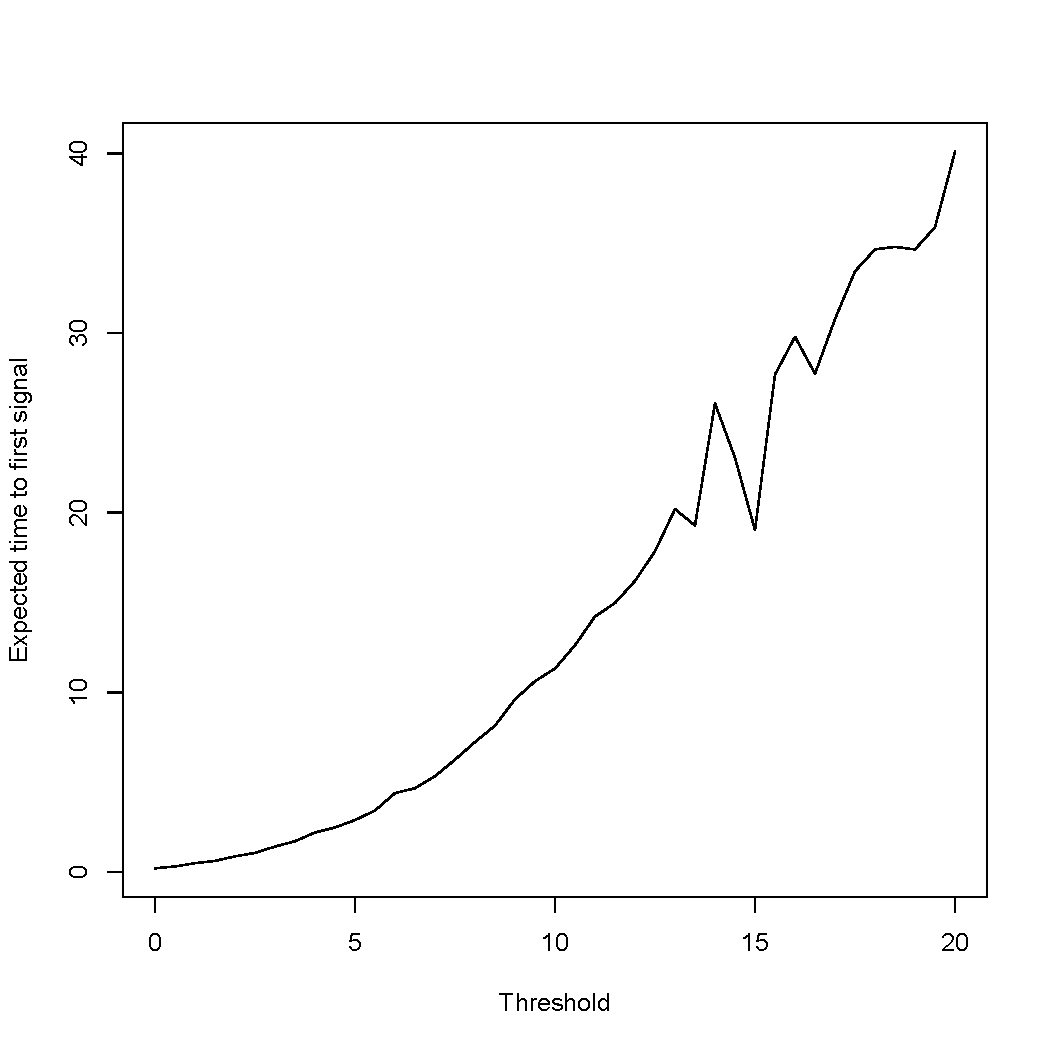
\includegraphics[width=\linewidth]{figures/expected_wait.pdf}

\subsection{Deterministic Analog}
\subsection{Simulation Methods}
Gillespie, Euler-Maruyama?
\section{Pairwise Dynamics}
\subsection{Deterministic Analysis}
\subsection{Effect of Threshold}
\subsection{Selection on Threshold}

\section{Network Dynamics}

\section{Discussion}

\section{Appendix}
\begin{fact}
If the probability of an event occurring in $[t,t+dt)$ is $rdt$ then the number of events occurring in a period of time of length $t$ is a Poisson random variable with mean $rt$, i.e. the probability of $n$ events occurring is 
$$P(n,t)=\frac{e^{-rt}(rt)^n}{n!}$$
\end{fact}
\begin{pf}
\end{pf}

\begin{fact}
$N(\lambda,t)$ is a Poisson random variable giving the number of events that happen in a time $t$ if events occur at a rate $\lambda$.  If, when one of those events occurs, it can be categorized as one of two mutually exclusive events which occur with probabilities $p_1,p_2$ with $p_1+p_2\leq 1$ and $N_i(p_i,\lambda,t)$ is the random variable giving the number of events categorized as $i$ in time $t$, then $N_1(p_i,\lambda,t),N_2(p_2,\lambda,t)$ are independent Poisson random variables with rates $p_1\lambda$ and $p_2\lambda$.
\end{fact}
\begin{pf}
To show that $N_1,N_2$ are independent it suffices to show that, for all $n,m\in\N$, $P(N_1=n,N_2=m)=P(N_1=n)P(N_2=m)$.
\end{pf}

\nocite{*}
\bibliographystyle{plain}
\bibliography{signaling_model}

\end{document}


